\documentclass[a4paper,12pts]{article}


\usepackage{francois-preamble}
\usepackage{hyperref}
\usepackage[english]{babel}
\usepackage[latin1]{inputenc}
\setlength{\textwidth}{14cm}
\setlength{\oddsidemargin}{1cm}

\begin{document}

\title{Assignment 4: Segmentation \\
Vision and Image Processing}
\author{ Fran\c{c}ois Lauze and S�ren Olsen}
\date{January 8, 2020}
\maketitle


\noindent 
This is the 4th mandatory assignment on the course Vision and Image Processing (5th with
quiz included). The goal is to implement some basic Segmentation algorithms and discuss
their results.  \bigskip

{\bf This assignment must be solved in groups}. We expect that you will
form small groups of 2 to 4 students that will work on this assignment.
You have to pass this and the other mandatory assignments in
order to pass the course. 
\bigskip

{\bf The deadline for this assignment is Wednesday 22/01, 2020 at 20:00}. 
You must submit your solution electronically via the Absalon home
page. For general information on relevant software, requirement to the form
of your solution including the maximal page limit, how to upload on
Absalon etc, please see the first assignment.

\section*{Segmentation}

The goal of this assignment is to implement two basic segmentation algorithms and a simple
post processing one.
\begin{enumerate}
\item The $k$-means algorithm for grey-scale images, first with $k=2$, then with larger $k$s,
  via Lloyd's algorithm. Handling scalar values should be easy!
\item The Otsu's thresholding algorithm (for a single threshold) following the description
  provided on the slides or the paper of N. Otsu which you can find in Absalon.
\item A cleaning/denoising algorithm, briefly described in the slides for removing small
  holes in the segmentations. At each \emph{interior pixel} compute how many of its
  neighbours are of a given label. If enough of them ``vote'' for a given label, this pixel
  (in the cleaned segmentation) is given the majority value. The threshold on the number
  of votes is a parameter of the algorithm. It could be: all neighbours, or 2/3 of them
  etc.
  
  \begin{center}
    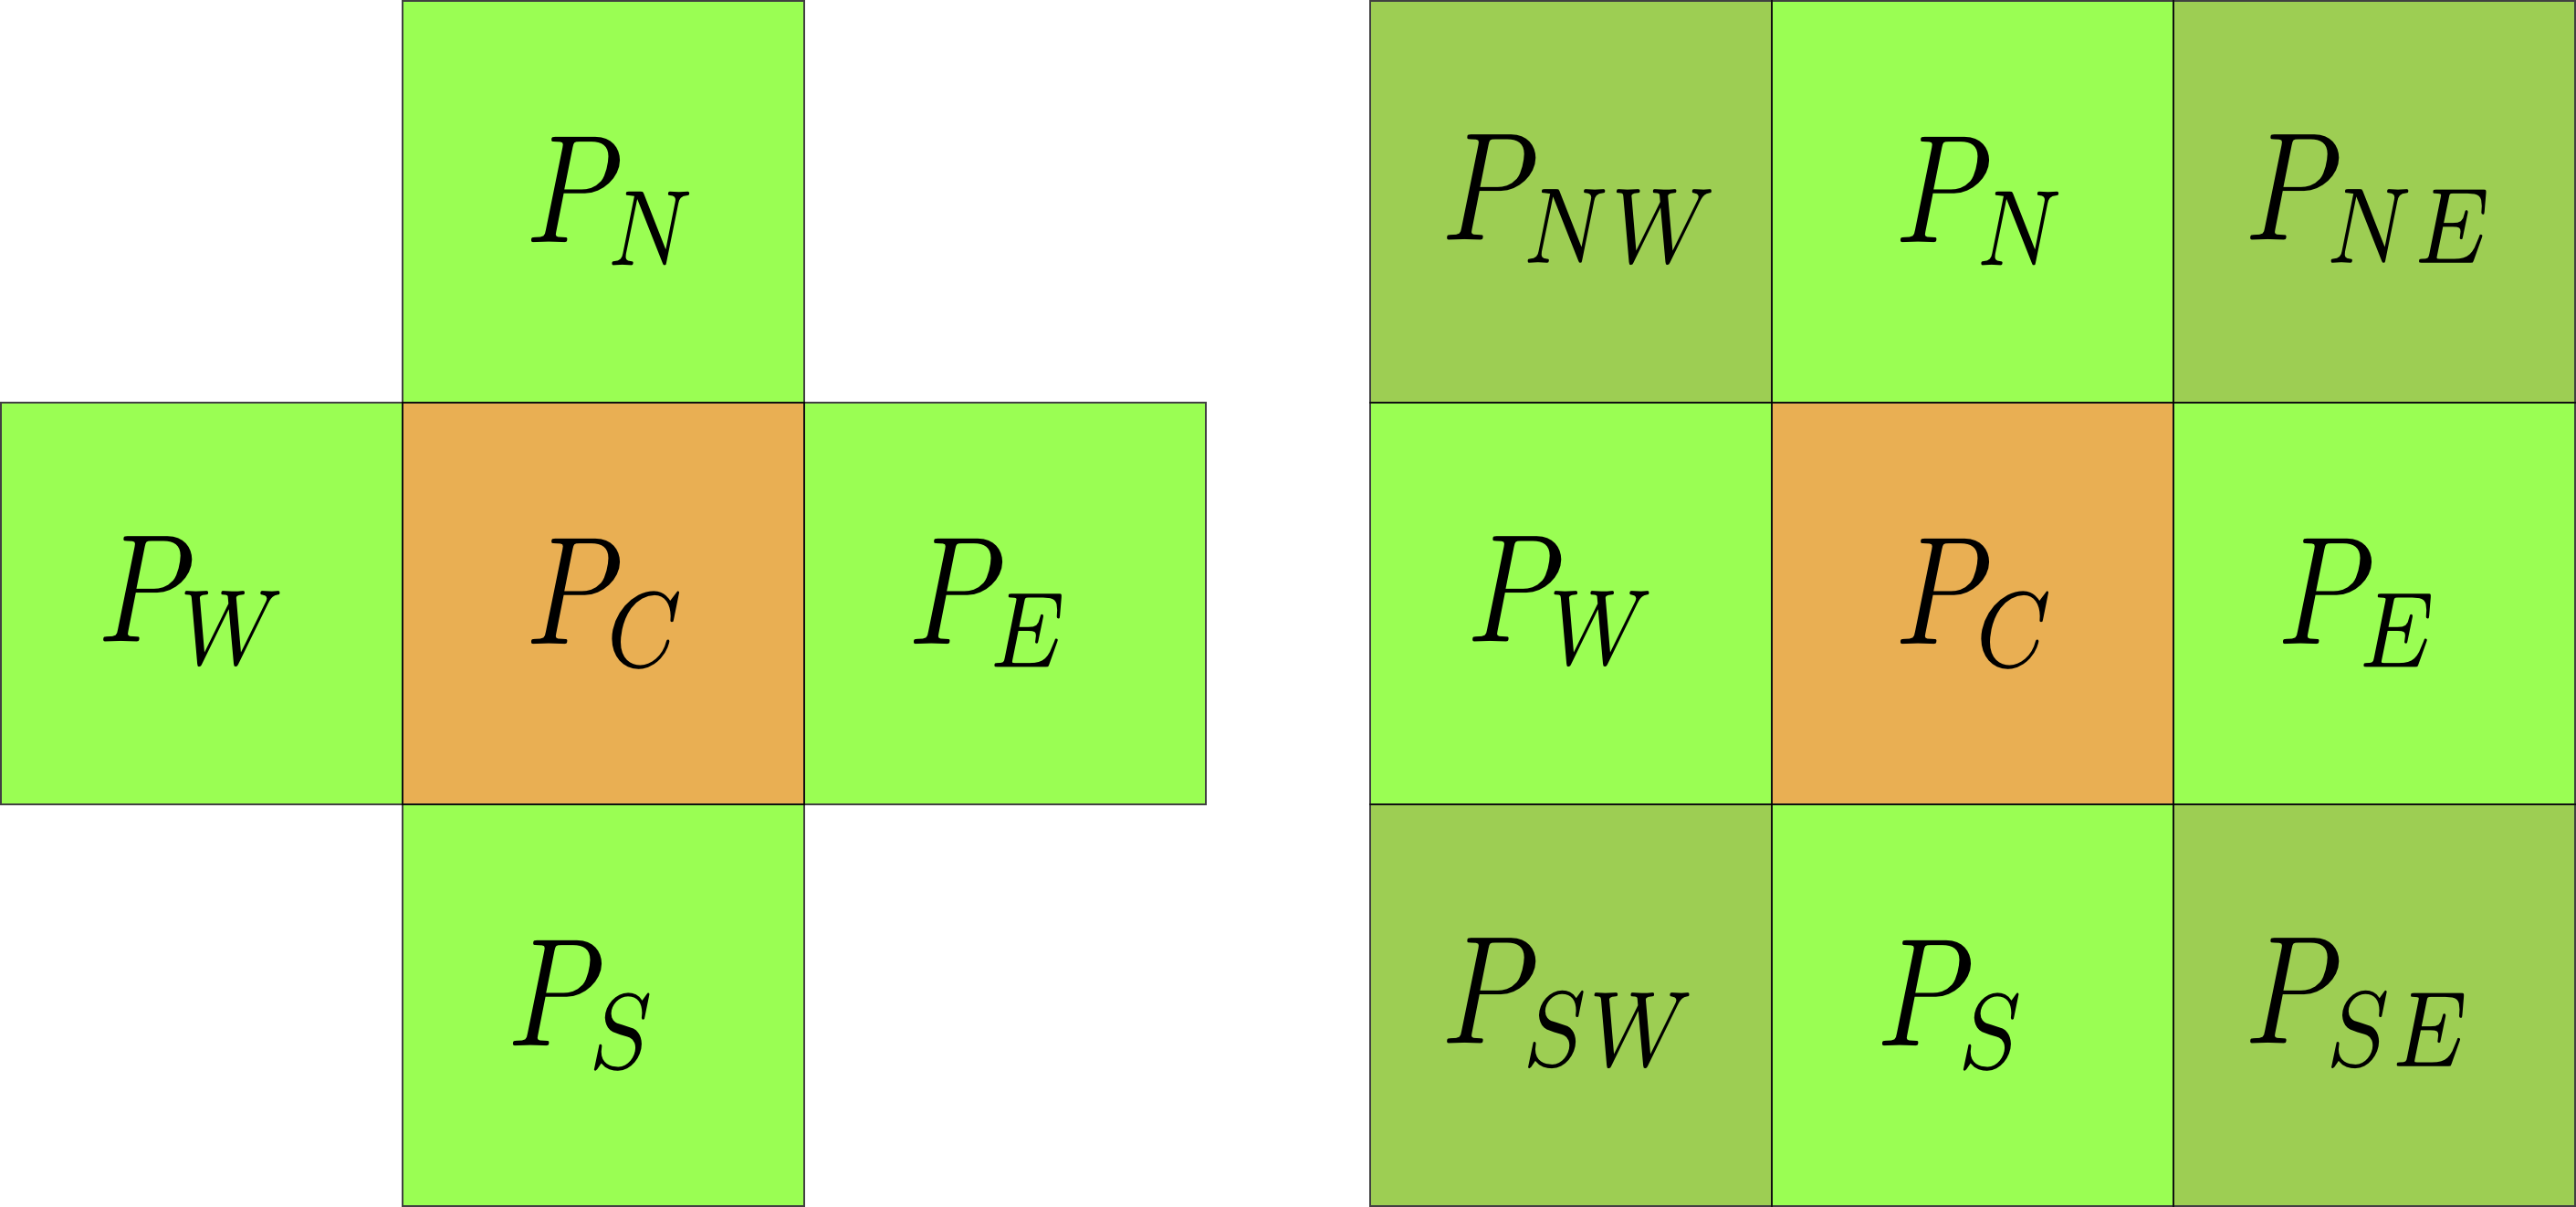
\includegraphics[width=0.5\textwidth]{FIGURES/neighborhoods}~\\
    4 and 8 pixels neighbourhood systems.
  \end{center}
  You will allow for either 4-pixels or 8-pixels neighbourhoods. It should be possible to
  iterate this algorithm a certain amount of time, and this should be a parameter in your
  implementation.
\end{enumerate}

~\\
You will use several images provided to you on Absalon in the \texttt{Assignment 4 data}
folder, and you are welcome to use other grey-scale images of your choice, or a colour one
that you convert to grey-scale.
~\\

\begin{itemize}
\item Run you implementations of $k$-means and Otsu on Absalon's images and one or more of your choice.
\item Comment on their similarity, dissimilarities?
\item Run several iterations of the segmentation denoising algorithm with varying voting
  thresholds values. Comment on the results.
\item Run a $k$-means segmentation with $k>2$. Can it help with the page image?
\item Can you imagine a way to
  generalise the segmentation denoising algorithm to more than 2 segments? Comment on it.
\item You may want to try some of the algorithms available in \texttt{scikit-learn}, such
  as the Chan-Vese segmentation.
\end{itemize}


\section*{Data}
Here are the 4 images provided to you for this assignment. Image 3, a
micro-tomographic slice of a rock sample, has been strongly reduced in size (the original
is 2560x2560 pixels).

\begin{center}
  \begin{tabular}[h]{c@{\hskip 5mm}c}
    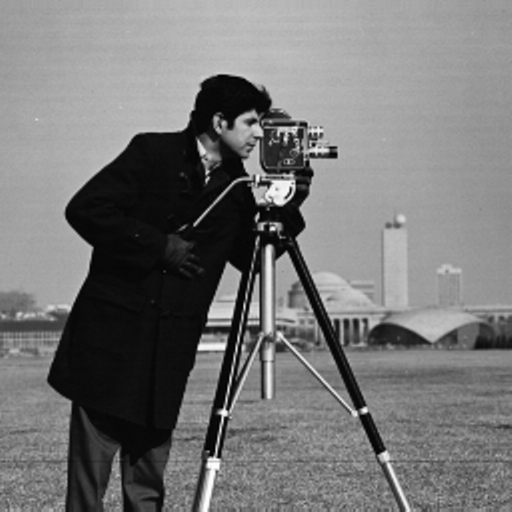
\includegraphics[width=0.2\textwidth]{DataCode4/camera} &
    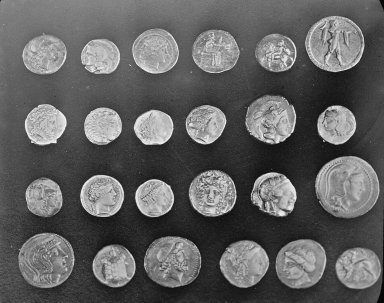
\includegraphics[width=0.2525\textwidth]{DataCode4/coins} \\ 
    Cameraman & Coins\\
    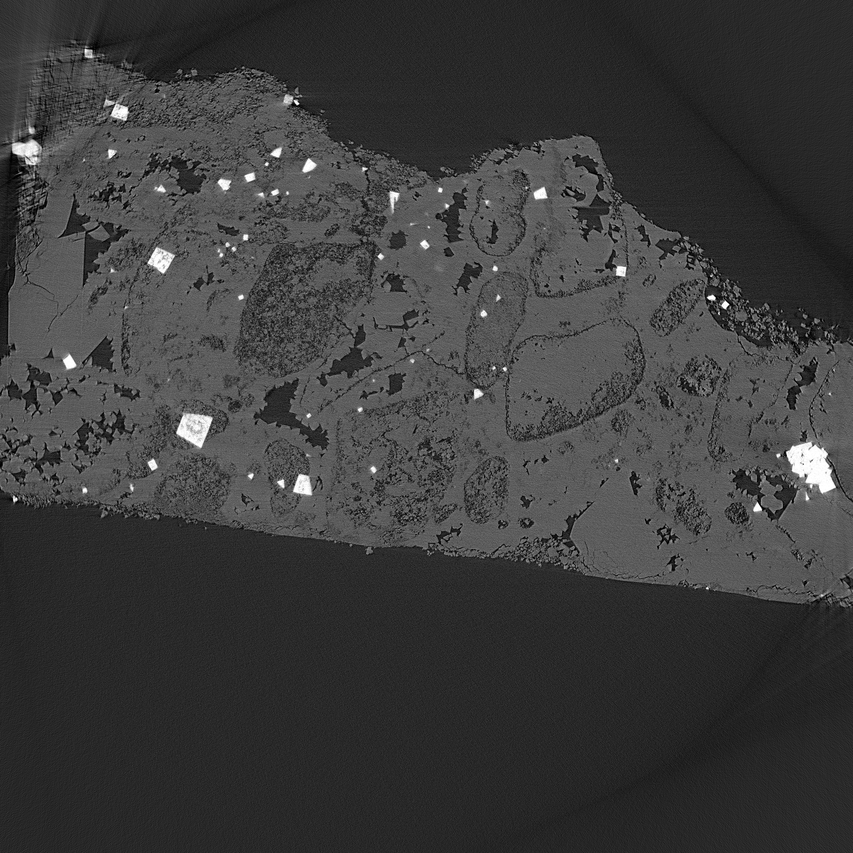
\includegraphics[width=0.2\textwidth]{DataCode4/rocksample} &
    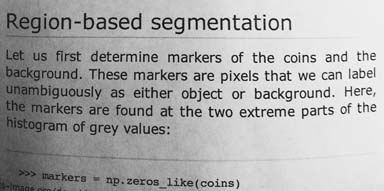
\includegraphics[width=0.25\textwidth]{DataCode4/page} \\
    rock sample slice & page
  \end{tabular}
\end{center}

\end{document}
